\chapter{Atomic physics: Experimental techniques and theory}\label{chap:atomic_physics}

\begin{itemize}
\item Descriptions of the relevant physics in atomic physics experiments: Doppler cooling and magneto-optical traps, Sisyphus cooling, dipole forces, Feshbach resonances, scattering theory, Bose–Einstein statistics. Show how the Hamiltonian of a `two level' (32 levels, all things considered for $^{87}$Rb D line) atom with fine structure, hyperfine structure and Zeeman splitting arises from consideration of the different angular momenta. Use this to derive the differential equations for the state populations of an atom in a driving laser field. Gross Pitaevskii equation for single species, dual species and spinor condensate.

\item{Doppler cooling}
\item{Magneto-optical trapping}
\item{Optical dipole trapping}
\item{Two-body scattering and Feshbach resonances}
\item{ -> Include stuff from 3rd year report}
\item{Spin, fine structure, and hyperfine structure}
\item{Equations of motion for two level atom with hyperfine structure}
\item{The Monte-Carlo wavefunction method}
\item{Mean field theory for Bose–Einstein condensates}
\item{ -> Superfluid velocity}
\item{ -> Vortices}

\end{itemize}
\section{Cooling, trapping, and manipulating atoms}
\textsc{Bec}s provide such a tantalising opportunity for studying quantum phenomena not only because of their interesting properties, but also because of the level of control they afford. Many of the same techniques which allow experimentalists such control over their creation are also employed in the creation thereof, and many were discovered along the way to Bose--Einstein condensation.

The main experimental techniques used to create \bec---and which we are and will be employing in that pursuit---are Doppler cooling, magneto-optical and dipole trapping, polarisation gradient (Sisyphus) cooling, and evaporative cooling.

These were discovered, perhaps by no coincidence, in roughly the same order as they are called for in a \bec\ experiment.

\subsection{Doppler cooling}

Doppler cooling, demonstrated in 1978 \cite{wineland_radiation-pressure_1978} is a consequence of the simple observation that atoms see the wavelength of incident light Doppler shifted depending on their velocity. This can be used to selectively transfer momentum to only fast-moving atoms, by tuning an incident laser slightly redder than would be required for a resonant absorption. If six lasers in counterpropagating pairs orthogonal to each other surround a cloud of atoms, the atoms can be cooled close to the \emph{Doppler limit} \cite[p 58]{metcalf_laser_1999}

\begin{equation}
k_\up{B} T_\up{D} = \frac{\hbar\Gamma}2
\end{equation}

where $\Gamma$ is the linewidth of the atomic transition. For the cooling transition used for Doppler cooling $^{87}$Rb\footnote{The D$_2$ line, $5\up{S}_{\frac12}\rightarrow$ $5\up{P}_{\frac32}$, approximately 780 nm.}, this gives $146\,\upmu$K, which is approximately a factor of a thousand too high for Bose-condensation. These atoms are also not trapped.

\subsection{Magneto-optical and magnetic trapping}

Magneto-optical trapping, first demonstrated in 1987 \cite{raab_trapping_1987} comes from the realisation that a magnetic field can be used to \emph{spatially} vary the detuning from resonance that the atoms in the above mentioned arrangement of lasers see. This is possible due to the Zeeman effect \cite{zeeman_influence_1897}, in which the wavelengths of atomic transitions are shifted in a magnetic field.

If a field profile can be found which causes the transition to come closer to resonance as the atoms move away from a central point, then it forms a trap---atoms  that stray too far from the center will absorb more strongly and be deflected back\footnote{The polarisations of the beams are such that absorption from the inward facing beam occurs, rather than from the one that would accelerate the atom further outward!}.

The field configuration used in an anti-Helmholtz one, with two coils opposite each other carrying opposing currents. The resulting magnetic field profile has a zero in the middle and increases in magnitude in all directions.

With the Doppler beams off, this magnetic field still provides a trapping potential, due to the magnetic dipole interaction:

\begin{equation}
V(\vec{r}) = -\vec \mu \cdot \vec B,
\end{equation}
where $\vec\mu$ is the atomic magnetic moment, and $\vec B$ the magnetic field. This only traps some atomic spin states, and has losses due to spin-flips \cite{brink_majorana_2006} near the field zero.

\subsection{Optical trapping}

Optical dipole trapping on the other hand relies on the \emph{dipole force}, in which off-resonant light shifts the energy of the eigenstates of the combined atom-light system, the so called \emph{dressed states}. This energy shift, called the \emph{light shift}, depends on the intensity of the light, and so results in a potential that spatially varies as the intensity of the light. In the limit of large detuning (compared to Rabi frequency), this shift is given by \cite[p 8]{metcalf_laser_1999}:

\begin{equation}
\Delta E = \frac{\hbar\Omega^2}{4\delta}
\end{equation}

where $\delta$ is the detuning from resonance and the Rabi frequency is:
\begin{equation}
\Omega=\frac{eE_0}\hbar\langle1|\vec{x}|2\rangle,
\end{equation}

where $E_0$ is the amplitude of the light's electric field and  $\langle1|\vec{x}|2\rangle$ is the dipole moment between the two states in a two-level system.

With the potential proportional to $E_0^2$, and thus the light's intensity, the force the atom experiences is proportional to the light's intensity gradient. For this reason, the dipole force is also called the \emph{gradient force}. The name \emph{dipole force} comes from the fact that the force can be equivalently understood to arise from the polarisability of atoms in a light field, giving rise to a force identical to that which traps polarisable materials in optical tweezers \cite{ashkin_acceleration_1970}.

\subsection{Polarisation gradient cooling}

Polarisation gradient cooling, also called Sisyphus cooling, was proposed in 1989 \cite{dalibard_laser_1989, ungar_optical_1989} to explain experimentally measured cold atom cloud temperatures \cite{lett_optical_1989} which, at \textsc{nist} in 1988, were found to be well below the expected limit obtainable by the well understood method of Doppler cooling\footnote{As well as to explain other discrepancies between experiments and the theory of Doppler cooling, such as the optimal detuning of light being much greater than predicted.}, one of the few examples of experiments turning out better than expected. A one dimensional theory has been developed \cite{dalibard_laser_1989} which has found remarkable agreement with three dimensional experiments \cite{salomon_laser_1990}

One common configuration for Sisyphus cooling comprises two counterpropagating laser beams in each spatial dimension, both linearly polarised but with their polarisation angles perpendicular to one another. The optical field resulting from the two beams' superposition has regions of linear polarisation and of both helicities of circular polarisation, and varies between them on a length scale shorter than an optical wavelength.

The effect on multi-level atoms as they move from regions of one circular polarisation to another is that they are pumped alternately from one extreme of their spin-projection states to the other, alternately climbing and descending potential hills due to the dipole forces from the regions of different polarisations\footnote{If you consider only one polarisation of light, its intensity varies sinusoidally in space, creating a series of potential hills and wells via the dipole force}. And so, like the Greek legend of Sisyphus\footnote{Polarisation gradient cooling is but one of a family of so called `Sisyphus cooling' methods, all of which involve atoms repeatedly climbing potential hills.}, who was doomed to push a rock uphill for eternity, the atoms are climbing hills repeatedly. Due to the state dependence of the strength of the dipole forces, the atoms climb steeper hills than they descend, and are thus slowed and cooled.

This type of cooling does not work in a magnetic field; the splitting of transition frequencies makes it impossible for an atom to traverse its spin manifold on one laser frequency. For this reason the Sisyphus cooling stage is performed with magnetic fields off, though a sufficiently short period is required such that the atoms can be recaptured when the trapping field is restored.

\subsection{Evaporative cooling}

The final stage of cooling is forced \textsc{rf} evaporative cooling \cite{hess_evaporative_1986, anderson_observation_1995}, which decreases the temperature of the cloud by systematically removing the hottest atoms. This is performed in a magnetic trap, which as mentioned earlier, only traps certain spin states. Evaporation proceeds by using an \emph{\rf\ knife} to induce spin flips in the atoms. The \textsc{rf} frequency is chosen such that is is only resonant with atoms some distance away from the center of the trap (via the Zeeman shift). The furthest out atoms are the most energetic, possessing the energy to climb the magnetic potential the furthest. By flipping their spins, these atoms are ejected due to the magnetic field becoming anti-trapping for them.

The cloud is given some time to rethermalise and the knife\footnote{So called because it cuts the tail off the velocity distribution of the atom cloud.} is moved inward where it removes slightly colder atoms. This is repeated until the desired compromise of lower temperature/lower atom number is reached. Usually some method is employed to prevent atoms near the center of the trap from undergoing spin flips \cite{brink_majorana_2006} as they move across the field zero. The method we'll employ is to use an optical dipole trap in combination with the magnetic trap \cite{lin_rapid_2009}, such that the coldest atoms get trapped in the dipole trap which is offset from the magnetic field zero.

\subsection{Feshbach resonances}

A Feshbach resonance \cite{chin_feshbach_2010} is an enhancement of the interparticle interaction strength when when a certain magnetic field strength is applied\footnote{Feshbach resonances can also be induced optically and with \rf\, but magnetic resonances are the most commonly used.}. This phenomenon was first discovered in ultracold atoms in 1998 \cite{inouye_observation_1998}, and is now a staple of cold atom experiments.

\begin{figure}%[htb]
\begin{center}
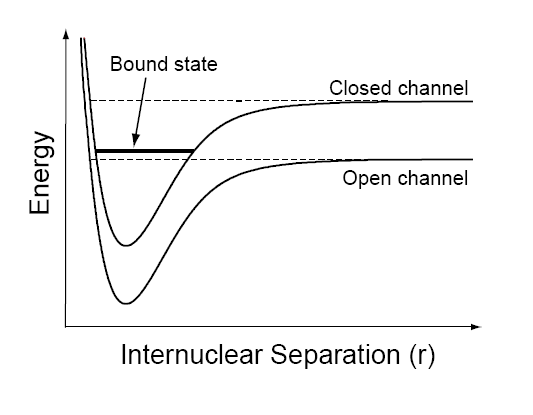
\includegraphics[width=0.5\textwidth]{figures/unsorted/feshbach.png}
\caption{When atoms approach each other with spins aligned, they are in the \emph{open channel}. In this channel they are unbound, but do not have enough energy to be free in the other channel - the \emph{closed channel}. In the close range however, the atoms may have energy corresponding to a bound (molecular) state of the closed channel, a resonance which causes a divergence in the scattering length. The energy difference between the two channels can be tuned with a magnetic field and so these resonances can be induced in a wide range of situations.}\label{fig:feshbach}
\end{center}
\end{figure}
The interparticle interaction mentioned above:

\begin{equation}
g = \frac{2\pi \hbar^2 a}{m_r}
\end{equation}
where $m_r$ is the reduced mass of a pair of the interacting particles, is dependent on a parameter $a$ called the \emph{s-wave scattering length}, which characterises low energy collisions between atoms. It is sensitive not only to what species of atoms are colliding, but also to their spin states. For each combination of spins, there is a different inter-atomic potential (called a \emph{channel}) which determines the collision dynamics (Figure \ref{fig:feshbach}).

The resulting scattering length is sensitive to any bound states of this inter-atomic potential which are near the collision energy. If the channels of different spin states are coupled via the hyperfine interaction\footnote{Requiring that the atoms in question have a nuclear magnetic moment.}, then the scattering length is also sensitive to bound states in the channels other the one the atoms are in when they are far from each other. Due to the Zeeman effect, the energies between the different channels can be shifted with a magnetic field, and so a bound state can be shifted close to the collision energy, which causes the scattering length to diverge.

The end result is that at certain magnetic field strengths we find that atoms are much more strongly attracted to or repelled from each other.

\begin{figure}%[htb]
\begin{center}
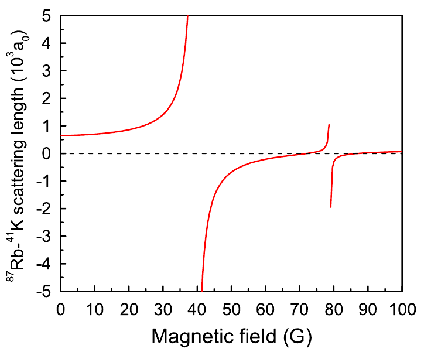
\includegraphics[width=0.5\textwidth]{figures/unsorted/feshKRb.png}
\caption{Predicted interspecies scattering length \cite{thalhammer_double_2008} as a function of magnetic field strength, for $^{41}$K and $^{87}$Rb both in their lowest energy hyperfine groundstate. The 35 gauss resonance is one of the main reasons for this pair of atoms being used in this project. It has a particularly low field strength and large width compared to most Feshbach resonances.}\label{fig:feshKRb}
\end{center}
\end{figure}

We plan to use a Feshbach resonance (Figure \ref{fig:feshKRb}) to enhance the interspecies repulsion between $^{87}$Rb and $^{41}$K, thus trapping tracer particles more strongly in vortex cores.


\section{Mean field theory: The Gross--Pitaevskii equation and vortices}

Bose-condensates are described well by \emph{mean field} theory, whereby the many-body wavefunction is approximated by a product of identical single-particle wavefunctions. Indeed, that the majority of the atoms are in the same quantum state is one of the defining features of \bec. The effect of interparticle interactions is included as a nonlinear term in the Schr\"odinger equation for the single particle wavefunctions, known as the Gross-Pitaevskii equation:

\begin{equation}
\frac{\partial \Psi}{\partial t} = \left[-\frac{\hbar^2}{2m}\nabla^2 + V(\vec{x}) + g|\Psi|^2\right]\Psi,
\end{equation}

where $g$ characterises the strength of the interparticle interactions\footnote{And is usually positive---having the effect of stabilising \bec s by self-repulsion.}, and $\Psi = \sqrt{N}\Psi_\up{single}$ is the single-particle wavefunction scaled by the square root of the number of particles\footnote{Thus giving it the property that $|\Psi|^2$ is the particle density.}.

In the hydrodynamic formulation of quantum mechanics \cite{madelung_quantentheorie_1927}, the flow velocity of a spatial wavefunction can be defined by considering the probability current to be a product of density and velocity. This allows us to define the superfluid velocity of a \bec\ as:
\begin{equation}
\vec v = \frac\hbar m \nabla\phi
\end{equation}
where $\phi$ is the phase of the condensate wavefunction $\Psi$. Integrating this velocity over any closed path $\gamma$ gives us the circulation:

\begin{align}
C &= \frac\hbar m\oint_\gamma\nabla\phi\,ds\\
  &= \frac\hbar m 2\pi n.\qquad n=0,1,2\dots
\end{align}
The fact that the circulation is quantised means that vorticity cannot exist in the condensate except in one-dimensional lines, about which the wavefunction's phase winds by a multiple of $2\pi$. These topological defects are the quantised vortices that are central to this project.

At a vortex core, the atom density of a \bec\ must go to zero. This can be intuitively understood to arise from centrifugal forces, but is also required in order for the wavefunction to be continuous and single-valued across the core. This drop in density in the vicinity of a vortex core is what our method exploits in order to trap atoms within the cores.

\section{Optical transitions on the $^{87}$Rb D line}

We atomic physicists do our theory work at an intermediate level of abstraction, at which many quantities and systems of interest can be computed and simulated with accurate models using standard quantum mechanics, but with the models not being fully a-priori. Instead, the Hamiltonians we feed to the machinery of standard quantum mechanics encapsulate some of the details we are not interested in or that are too hard to compute, with the link between the underlying layers of reductionism and the higher layer usually provided by experimentally measured constants rather than calculations from fundamental physics. In this way we can readily compute results about the atoms we are interested in by treating them as simpler systems than they actually are, with some of the the underlying details encapsulated by terms in an effective Hamiltonian for the dynamics that we are interested in.

In this section I'll summarise what the $^{87}$Rb \textsc{d} line looks like from the perspective of a cold atom physicist, building up a Hamiltonian containing all 32 sublevels of the ground and first excited state of $^{87}$Rb including fine structure, hyperfine structure, interaction with a magnetic field, and optical transitions between states. This Hamiltonian is the starting point for any calculations regarding cooling, trapping, and coherent control of $^{87}$Rb, and the process for other alkali earth metals is much the same.

\subsection{Fine structure}

The rubidium 87 D line is not just one transition between a ground state and an excited state---there are two excited states, and the two resulting transitions are called, in order of their transition frequencies, the $\up{D}_1$ and  $\up{D}_2$ lines. Thus the ground and first excited state of $^{87}$Rb are actually a ground state plus two non-degenerate excited states, once we take into account fine structure. The groundstate is an $S$ state (electronic orbital angular momentum quantum number $L=0$), called the $S_{\frac12}$ state, and the two excited states are $P$ states $(L=1)$, one with the electron spin anti-aligned with its orbital angular momentum ($J=1/2$) and one with the electron spin aligned with its orbital angular momentum ($J=3/2$), called the $P_{\frac12}$ and $P_\frac32$ states respectively. In all of these states, $^{87}$Rb's single outer-shell electron occupies an orbital with principle quantum number $n=5$, which for brevity we leave out of the notation. The transition between $S_{\frac12}$ and $P_{\frac12}$ is called the $\up{D}_1$ line, with experimentally measured (angular) transition frequency $\omega_{\up{D}_1}$, and the transition between $S_{\frac12}$ and $P_{\frac32}$ is the $\up{D}_2$ line with angular transition frequency $\omega_{\up{D}_2}$. These transition frequencies correspond to optical wavelengths of $\lambda_{\up{D}_1} \approx 795\unit{nm}$ and $\lambda_{\up{D}_2} \approx 780\unit{nm}$\cite{steck_rubidium_2010}.

This fine structure is treated entirely empirically for our purposes, and so our base Hamiltonian for the rubidium D line, taking into account only fine structure, is simply a statement of the experimentally measured energy differences between the states:

\begin{align}
\hat H_0 = \hat 0_{S_{1/2}} \oplus
\hbar\omega_{\textsc{D}_1} \hat1_{P_{1/2}} \oplus
\hbar\omega_{\textsc{D}_2} \hat1_{P_{3/2}},
\end{align}

where $\hat 0_{S_{1/2}}$, $\hat1_{P_{1/2}}$, and $\hat1_{P_{3/2}}$ are zero and identity operators each acting on the subspace of states within the $S_{\frac12}$, $P_{\frac12}$, or $P_{\frac32}$ manifold, and $\oplus$ is the direct sum.\footnote{Not to be confused with the Kronecker sum, with which it shares notation. The direct sum concatenates matrices as blocks, producing a larger, block-diagonal matrix with dimension equal to the \emph{sum} of the dimensions of the matrices being direct-summed, whereas the Kronecker sum is the the regular sum of matrices after each has been multiplied using the Kronecker-product with identity matrices with sizes of the other matrices in the sum, producing matrices with dimension equal to the \emph{product} of those being summed.} The matrix representation $H_0$ of $\hat H_0$ in the basis in which it is diagonal is
\begin{align}
& H_0  = 
\left[\begin{matrix}
    \left[\begin{smallmatrix}\ddots &&\\&0&\\&&\ddots\\\end{smallmatrix} \right]\\
    & \left[\begin{smallmatrix}\ddots &&\\&\hbar\omega_{\textsc{D}_1}&\\&&\ddots\\\end{smallmatrix} \right]\\
    & &\left[\begin{smallmatrix}\ddots &&\\&\hbar\omega_{\textsc{D}_2}&\\&&\ddots\\\end{smallmatrix} \right]
\end{matrix} \right],
\end{align}
which is a block-diagonal matrix with each block also being a diagonal matrix. We have not yet specified the size of each submatrix---the size of each differs and depends on how many hyperfine and Zeeman sublevels are in that state.

This base Hamiltonian is worth pointing out since the energy differences between its three states are orders of magnitude larger than any of the energy differences between hyperfine and Zeeman sublevels within them. When doing any sort of calculations or simulations then, this time-independent Hamiltonian can be removed from the equations using an interaction picture, which we will come to shortly when we discuss optical transitions. 

\subsection{Hyperfine structure}

Within each of the $S_{1/2}$, $P_{1/2}$ and $P_{3/2}$ states, the single outer-shell electron's total angular momentum $\hat {\vec J}$ has an interaction with $^{87}$Rb's nuclear angular momentum $\hat{\vec I}$. This results in multiple discrete energy levels depending on the relative orientation of the two separate angular momenta. The interaction Hamiltonian for this hyperfine structure is [cite steck and the two references steck cites]\footnote{Note that this expression differs from those in the cited references by a factor of $1/\hbar^2$---this is because I define the $\hat{\vec I}$ and $\hat{\vec J}$ angular momentum operators in SI units, rather than in units of $\hbar^2$.}:
\begin{align}\label{eq:H_hfs}
\hat H_\up{hfs} = \frac{A_\up{hfs}}{\hbar^2} \hat{\vec I} \cdot \hat {\vec J}
+ \frac{B_\up{hfs}}{\hbar^2}\frac
{3(\hat{\vec I}\cdot\hat{\vec J})^2 + \frac32 \hat{\vec I}\cdot\hat{\vec J} - I(I + 1)J(J + 1)}
{2I(2I - 1)J(2J - 1)},
\end{align}
where $J$ is the total angular momentum quantum number of the electron, equal to either $\frac12$ or $\frac32$ depending on which state in the D line we are considering, $I=\frac32$ is the total angular momentum quantum number of the nucleus, and $A_\up{hfs}$ and $B_\up{hfs}$ are empirically determined coupling constants. Here we see the boundary between the quantities we can calculate with the machinery of quantum mechanics and those that we cannot and need to determine empirically---this expression applies so long as $J$ and $I$ are good quantum numbers,\footnote{$J$ is a good quantum number so long as the hyperfine splitting is small compared to the spacing between the three states of the D line, which it is, and $I$ is a good quantum number so long as the hyperfine splitting is small compared to the energy difference between the groundstate and the first \emph{nuclear} excited state, which it most certainly is.} and the two terms are the dipolar and quadrupolar interactions [cite the review article] between two angular momenta, with the coupling constants determined empirically and encapsulating many details that are difficult to compute a-priori, such as relativistic effects and the exact shape of the electron orbitals given the presence of inner shell electrons. For the spherically-symmetric $S_{1/2}$ groundstate, there is no quadrupolar interaction and so $B_\up{hfs}$ is only nonzero for the two $P$ excited states.\footnote{The quadrupolar term should be explicitly excluded from numerical computations of the hyperfine splitting on the $S_{1/2}$ state, as it contains a division by zero in this case, which may lead to erroneous results even if the term is subsequently multiplied by $B_\up{hfs}=0$.} The values of $A_\up{hfs}$ and $B\up{hfs}$ for each of the three states of the D line can be found in [steck].

For a given state of the D line, we can construct the matrix representation $H_\up{hfs}$ of $\hat H_\up{hfs}$ in the basis in which the $z$ vector components $\hat{I}_z$ and $\hat{J}_z$ of $\hat{\vec I}$ and $\hat{\vec J}$ are diagonal by constructing matrix representations $\vec I_{\mathcal{I} \times \mathcal{J}}$ and $\vec J_{\mathcal{I} \times \mathcal{J}}$ of the operators $\hat{\vec I}$ and $\hat{\vec J}$ in that basis and then applying the expression (\ref{eq:H_hfs}). The subscript ${\mathcal{I} \times \mathcal{J}}$ on each of the matrices indicates that the matrix  is a representation of its respective operator in the product space of the spaces $\mathcal{I}$ and $\mathcal{J}$ of the two individual nuclear and electronic angular momentum degrees of freedom.

To construct matrix representations of angular momentum operators in the product space ${\mathcal{I} \times \mathcal{J}}$, we first need their matrix representations $\vec I_{\mathcal{I}}$ and $\vec J_{\mathcal{J}}$ in their respective subspaces, which we will write as $\vec I$ and $\vec J$ for brevity. We can then expand the two operators into the total space by applying a Kronecker product with an appropriate identity matrix to each:
\begin{align}\label{eq:kronecker_identity_I}
\vec I_{\mathcal{I} \times \mathcal{J}} &= \vec I \otimes \mathbb{I}_{\mathcal{J}}\\
\label{eq:kronecker_identity_J}
\vec J_{\mathcal{I} \times \mathcal{J}} &= \mathbb{I}_{\mathcal{I}} \otimes \vec J
\end{align}
where $\mathbb{I}_{\mathcal{I}}$ is the matrix representation of the identity operator on the $\mathcal{I}$ subspace, equal to a $(2I+1)\times(2I+1)$ identity matrix, with $\mathbb{I}_{\mathcal{J}}$ defined similarly. Each of the two matrices is actually a vector of matrices, one for the angular momentum projection in each of the directions $x$, $y$ and $z$. The procedure for constructing such matrices for arbitrary total angular momentum quantum numbers is as follows.\footnote{This explicit procedure for constructing the matrix representations of these operators is useful for entering into a programming language to produce programs capable of performing atomic physics calculations for arbitrary total angular momentum quantum number $J$, without having to explicitly enter the angular momentum operators for each value of $J$, which can be tedious and prone to human error.} I'll show the procedure for constructing $J_x$, $J_y$ and $J_z$ only for an arbitrary $J$, the procedure is identical for computing the vector components of $\vec I$.

For a given total angular momentum quantum number $J$, the vector components of $\vec J$ in the $z$ basis (the basis in which $J_z$ is diagonal) can be constructed using the raising and lowering operators $\hat J_+$ and $\hat J_-$. Since the action of the raising and lowering operators on an eigenstate of $J_z$ with angular momentum projection quantum number $m_J$ is to produce an adjacent ($m_J \pm 1$) eigenstate multiplied by a known constant [CITE SOME TEXTBOOK], this fact can be used to compute the nonzero matrix elements of $\hat J_+$ and $\hat J_-$ in the $\{\ket{m_J}\}$ basis:

\begin{align}
\matrixel{m_J}{\hat J_+}{m_J + 1} &= \hbar\sqrt{J(J + 1) - m_J(m_J + 1)}, \qquad m_J < J,\\
\matrixel{m_J}{\hat J_-}{m_J - 1} &= \hbar\sqrt{J(J + 1) - m_J(m_J - 1)}, \qquad m_J > -J,\\
\end{align}
and therefore compute explicit matrices for $J_+$ and $J_-$ in the $\{\ket{m_J}\}$ basis:\footnote{We're using the standard convention of ordering the eigenvectors $\{\ket{m_J}\}$ in descending order of $m_J$. This is at odds with the computer programming convention of looping over most indices in ascending order, and so care should be taken when constructing these matrices in a computer program.}
\begin{align}
J_+ &=
\left[\begin{smallmatrix}
    0 & \hdots \\
    \matrixel{J - 1}{\hat J_+}{J} & 0 & \hdots\\
    0 & \matrixel{J - 2}{\hat J_+}{J - 1} & 0 & \hdots\\
    \hdots & 0 & \matrixel{J - 3}{\hat J_+}{J - 2} & 0 & \hdots\\
    & & \ddots & \ddots & \ddots\\
    & & \hdots & 0 & \matrixel{-J}{\hat J_+}{-J + 1} & 0 \\
\end{smallmatrix} \right],\\
J_- &=
\left[\begin{smallmatrix}
0 &  \matrixel{J}{\hat J_-}{J - 1} & 0 & \hdots\\
\hdots & 0 & \matrixel{J - 1}{\hat J_-}{J - 2} & 0 & \hdots\\
& & \ddots & \ddots & \ddots\\
 & & \hdots & 0 & \matrixel{ -J + 2}{\hat J_-}{-J + 1} & 0\\
 & & & \hdots & 0 & \matrixel{ -J + 1}{\hat J_-}{-J}\\
 & & & & \hdots & 0\\
\end{smallmatrix} \right],
\end{align}
both of which have nonzero values along only one non-main diagonal adjacent to the main diagonal, and which form a Hermitian conjugate pair (or indeed, a transpose pair, since all elements are real). The matrix representations of $\hat J_x$ and $\hat J_y$ can then be computed by rearranging the defining expressions [CITE] for $\hat J_+$ and $J_-$;
\begin{align}
\hat J_+ = \hat J_x + \ii \hat J_y,\\
\hat J_- = \hat J_x - \ii \hat J_y,
\end{align}
for $\hat J_x$ and $\hat J_y$, and then applying the result to our matrix representations of $\hat J_+$ and $\hat J_-$ to obtain matrix representations $J_x$ and $J_y$ of $\hat J_x$ and $\hat J_y$ in the $\{\ket{m_J}\}$ basis:
\begin{align}
J_x &= \frac{J_+ + J_-}{2},\\
J_y &= \frac{J_+ - J_-}{2\ii}.
\end{align}
Finally, since $\{\ket{m_J}\}$ is the eigenbasis of $J_z$ with eigenvalues $\{\hbar m_J\}$, the matrix representation of $J_z$ is simply the diagonal matrix of eigenvalues:
\begin{align}
J_z = \left[\begin{smallmatrix}
\hbar J\\
& \hbar (J - 1)\\
& & \ddots\\
& & & \hbar (- J + 1)\\
& & & & -\hbar J\\
\end{smallmatrix} \right].
\end{align} 
We can also construct the matrix representation $J^2$ of the total (squared) angular momentum operator $\hat J^2$ as
\begin{align}
J^2 = J_x^2 + J_y^2 + J_z^2, 
\end{align} 
or equivalently
\begin{align}
J^2 = J(J+1)\hbar^2 \mathbb{I}_{\mathcal{J}},
\end{align}
since every $m_J$ state is an eigenstate of the $J^2$ operator with eigenvalue $J(J+1)\hbar^2$.

The above prescription can be used to produce matrix representations of angular momentum operators $J_x$, $J_y$, $J_z$ and $J^2$ for any integer or half-integer total angular momentum quantum number $J$. The three components can be considered a vector of matrices, $J$ for the vector angular momentum operator $\hat J$. Below is a Python function that computes these matrices as well as the corresponding eigenvectors:

\python{code_listings/angular_momentum_operators.py}

Using the above prescription to construct a matrix representation of the $\hat J$ operator with $J=\frac12$ for the $S_{1/2}$ and $P_{1/2}$ states, or $J=\frac32$ for the $P_{3/2}$ state, and to construct a matrix representation of the $\hat I$ operator with $I=\frac32$, we are close to being able to explicitly construct a matrix representation of the hyperfine interaction Hamiltonian for any state of the $^{87}$Rb D line. The remaining step is to obtain the matrix representations of the two operators in the $\mathcal{I}\times\mathcal{J}$ product space using \eqref{eq:kronecker_identity_I} and \eqref{eq:kronecker_identity_J}, and then we can apply \eqref{eq:H_hfs} to our matrices to obtain the matrix representation $H_\up{hfs}$ of $\hat H_\up{hfs}$ for a given $J$ corresponding to one of the three states on the D line:
\begin{align}\label{eq:H_hfs_matrix}
H_\up{hfs} = \frac{A_\up{hfs}}{\hbar^2}
\vec I_{\mathcal{I}\times\mathcal{J}} \cdot
\vec J_{\mathcal{I}\times\mathcal{J}}
+ \frac{B_\up{hfs}}{\hbar^2}\frac
{3(\vec I_{\mathcal{I}\times\mathcal{J}}\cdot
\vec J_{\mathcal{I}\times\mathcal{J}})^2
+ \frac32 \vec I_{\mathcal{I}\times\mathcal{J}}\cdot
\vec J_{\mathcal{I}\times\mathcal{J}}
 - I(I + 1)J(J + 1)}
{2I(2I - 1)J(2J - 1)},
\end{align}
where the products of vector components within the dot products are computed with ordinary matrix multiplication. Alternatively, one can use the matrices in their individual subspaces rather than their equivalents in the product space, so long as one interprets the dot products as ``Kronecker dot products":
\begin{align}\label{eq:H_hfs_matrix_kron}
H_\up{hfs} = \frac{A_\up{hfs}}{\hbar^2}
\vec I \krondot \vec J
+ \frac{B_\up{hfs}}{\hbar^2}\frac
{3(\vec I \krondot \vec J)^2
+ \frac32 \vec I \krondot \vec J
 - I(I + 1)J(J + 1)}
{2I(2I - 1)J(2J - 1)},
\end{align}
where $\krondot$ is the Kronecker dot product:
\begin{align}
\vec I \krondot \vec J \equiv I_x \otimes J_x + I_y \otimes J_y + I_z \otimes J_z.
\end{align}

In the above way one can construct an explicit matrix representation $H_\up{hfs}$ for the hyperfine interaction for a given state of the D line. But what basis is it in? Because the matrix representations $\vec I$ and $\vec J$ of the electron and nuclear angular momentum operators were constructed in the $\{\ket{m_I}\}$ and $\{\ket{m_I}\}$ bases of their respective subspaces $\mathcal{I}$ and $\mathcal{J}$, the matrices we have constructed in the product space $\mathcal{I}\times\mathcal{J}$ are in the basis $\{\ket{m_I}\} \times \{\ket{m_I}\}$---the direct product of the two sets of basis vectors for the separate subspaces, with elements:
\begin{align}
\{\ket{m_I}\} \times \{\ket{m_J}\} = \left\{\ket{m_I} \otimes \left.\ket{m_J} \ \right| \ \ket{m_I} \in \{\ket{m_I}\}, \ket{m_J} \in \{\ket{m_J}\}\right\},
\end{align}
where $\otimes$ is the direct product of vectors.\footnote{Although the symbol $\otimes$ is used for both the Kronecker product and the direct product (of vectors), the direct product applies to vectors/state vectors, and the Kronecker product to matrices/operators. The direct product also applies to basis sets/spaces, but with the symbol $\times$. I would prefer nomenclature refer to them all with the same name and symbol, especially since the result of a direct product applied to an $N$-element column vector and an $M$-element column vector is identical to that of applying a Kronecker product to an $N\times1$ matrix and a $M\times 1$ matrix, but I'll stick to the standard nomenclature.}

The representation of a state vector in this basis has elements:
\begin{align}
\vec \psi = 
\end{align}

\subsection{Zeeman sublevels}